\documentclass[a4paper,12pt]{article}
\usepackage[utf8]{inputenc}
\usepackage{geometry}
\usepackage{graphicx}
\usepackage{hyperref}
\geometry{margin=1in}

\title{Data Report: Exploring the Relationship Between Air Quality and Respiratory Health}
\author{}
\date{}

\begin{document}

\maketitle

\section*{Question}
The main question driving this project is:  
\textbf{How does air quality impact respiratory health across different regions in California, and what trends can be observed over time?}  
This study explores the relationship between pollution levels (PM2.5) and respiratory conditions, leveraging publicly available datasets.

\section*{Data Sources}

\subsection*{Air Quality Data}
\textbf{Source:} \href{https://aqs.epa.gov/aqsweb/documents/data_api.html}{EPA Air Quality System (AQS)}  
\textbf{Reason for Selection:} Provides detailed PM2.5 pollution measurements across California, critical for understanding environmental health impacts.  
\textbf{Content:} Includes pollutant levels, sampling locations, dates, and measurement units.  
\textbf{Structure and Quality:}
\begin{itemize}
    \item Structured tabular data with attributes such as \texttt{state\_code}, \texttt{date\_local}, \texttt{sample\_measurement}.
    \item Missing values handled during preprocessing.
    \item High reliability as data is maintained by the EPA.
\end{itemize}
\textbf{License and Obligations:}  
Licensed under open access by the EPA. Obligations include attribution, addressed in the project documentation.  
\href{https://data.gov/open-gov/}{License Details}

\subsection*{Respiratory Health Data}
\textbf{Source:} \href{https://data.cdc.gov/Chronic-Disease-Indicators/U-S-Chronic-Disease-Indicators/hksd-2xuw}{CDC Chronic Disease Indicators Dataset}  
\textbf{Reason for Selection:} Provides health metrics for respiratory conditions (e.g., asthma) at state and county levels.  
\textbf{Content:} Includes respiratory health indicators, demographic stratifications, and annual statistics.  
\textbf{Structure and Quality:}
\begin{itemize}
    \item Structured tabular data with fields such as \texttt{topic}, \texttt{state\_code}, \texttt{respiratory\_value}, and \texttt{year}.
    \item Data contains noise, requiring filtering for relevant indicators.
\end{itemize}
\textbf{License and Obligations:}  
Open Data license with attribution requirements, fulfilled via documentation.  
\href{https://opendatacommons.org/licenses/odbl/1-0/}{License Details}

\section*{Data Pipeline}

\textbf{Overview:}  
The pipeline automates data fetching, cleaning, transformation, merging, and output, consisting of the following stages:
\begin{enumerate}
    \item \textbf{Extraction:} Fetches air quality data via the EPA API and respiratory data from the CDC dataset, saved as raw CSV files.
    \item \textbf{Transformation:}
    \begin{itemize}
        \item \textbf{Air Quality Data:} Handled missing/negative values, converted date formats, and replaced numeric state codes with state abbreviations.
        \item \textbf{Respiratory Data:} Filtered for relevant topics (e.g., asthma), renamed columns for consistency, and standardized date formats.
    \end{itemize}
    \item \textbf{Loading and Analysis:} Merges datasets using \texttt{state\_code} and \texttt{year} as keys and outputs a merged CSV file for further analysis.
\end{enumerate}

\textbf{Pipeline Diagram:}
\begin{figure}[h!]
    \centering
    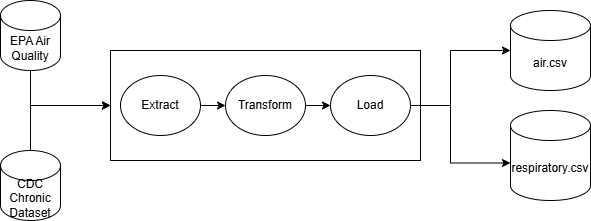
\includegraphics[width=\textwidth]{pipeline.png}
    \caption{Data Pipeline Diagram}
    \label{fig:pipeline}
\end{figure}

\textbf{Technology:}
\begin{itemize}
    \item \textbf{Language:} Python
    \item \textbf{Libraries:} \texttt{pandas}, \texttt{numpy}, \texttt{requests}, \texttt{threading}
\end{itemize}

\textbf{Issues and Resolutions:}
\begin{itemize}
    \item \textbf{Inconsistent column names across datasets:} Renamed columns to align (\texttt{state\_code}, \texttt{year}).
    \item \textbf{Numeric state codes in air quality data:} Converted to abbreviations (e.g., \texttt{6} to \texttt{CA}).
    \item \textbf{Mismatched keys during merging:} Standardized key columns before merging.
\end{itemize}

\textbf{Meta-quality Measures:}
\begin{itemize}
    \item Exceptions raised for missing or malformed data, with logs for progress.
    \item Dynamic column validation ensures compatibility with changes in data structure.
\end{itemize}

\section*{Result and Limitations}

\textbf{Output Data:}  
The pipeline produces a merged dataset (\texttt{merged\_data.csv}) containing air quality metrics and respiratory health data for California.  

\textbf{Data Quality:}
\begin{itemize}
    \item Cleaned and structured for analysis.
    \item Limitations include missing historical data for specific counties and aggregation obscuring localized trends.
\end{itemize}

\textbf{Output Format:}
\begin{itemize}
    \item \textbf{Format:} CSV for compatibility with analysis tools.
    \item \textbf{Reason:} Simple, universal format for structured data.
\end{itemize}

\textbf{Critical Reflection:}
\begin{itemize}
    \item While the datasets provide a solid basis for analysis, their granularity limits deeper insights into regional disparities.
    \item Incorporating additional datasets, such as socioeconomic indicators, could enhance the depth of analysis.
\end{itemize}

\end{document}
